\subsection{Genotype Size \& Genotype mutations}
Figure~\ref{fig:Size} shows genotype size under the various study conditions. The size is bounded (50 is the maximum size) and it limits the differences between those environments as most simulations converge towards this limit, however, one can clearly see here that \emph{Short-cycle Fluctuation} restrict the size of the genotypes while other forms of fluctuations do not appear to have any effect on genotype size. This size reduction could be a way to increase the impact of genotypic mutations on the phenotype. Indeed even if in LGP, when a mutation occurs, its effect is proportional to the size of the genotype, long genotype may enable redundancy information to stabilize the phenotype. Figure~\ref{fig:Size} depicts the amount of accumulated mutation of the most common individual. The amount of mutations separating the current most common individual from individuals created at initialization of the simulation. It is not surprising that more mutations are selected when there are environmental fluctuations\footnote{And those seem to depend more on the strength of these fluctuations than on their periodicity.} but we note that the proximity of strong fluctuation and Short Cycle fluctuations indicates that their genotype difference in size is not only explained by differences in the number of selected mutations.


\begin{figure}[h]
\centering
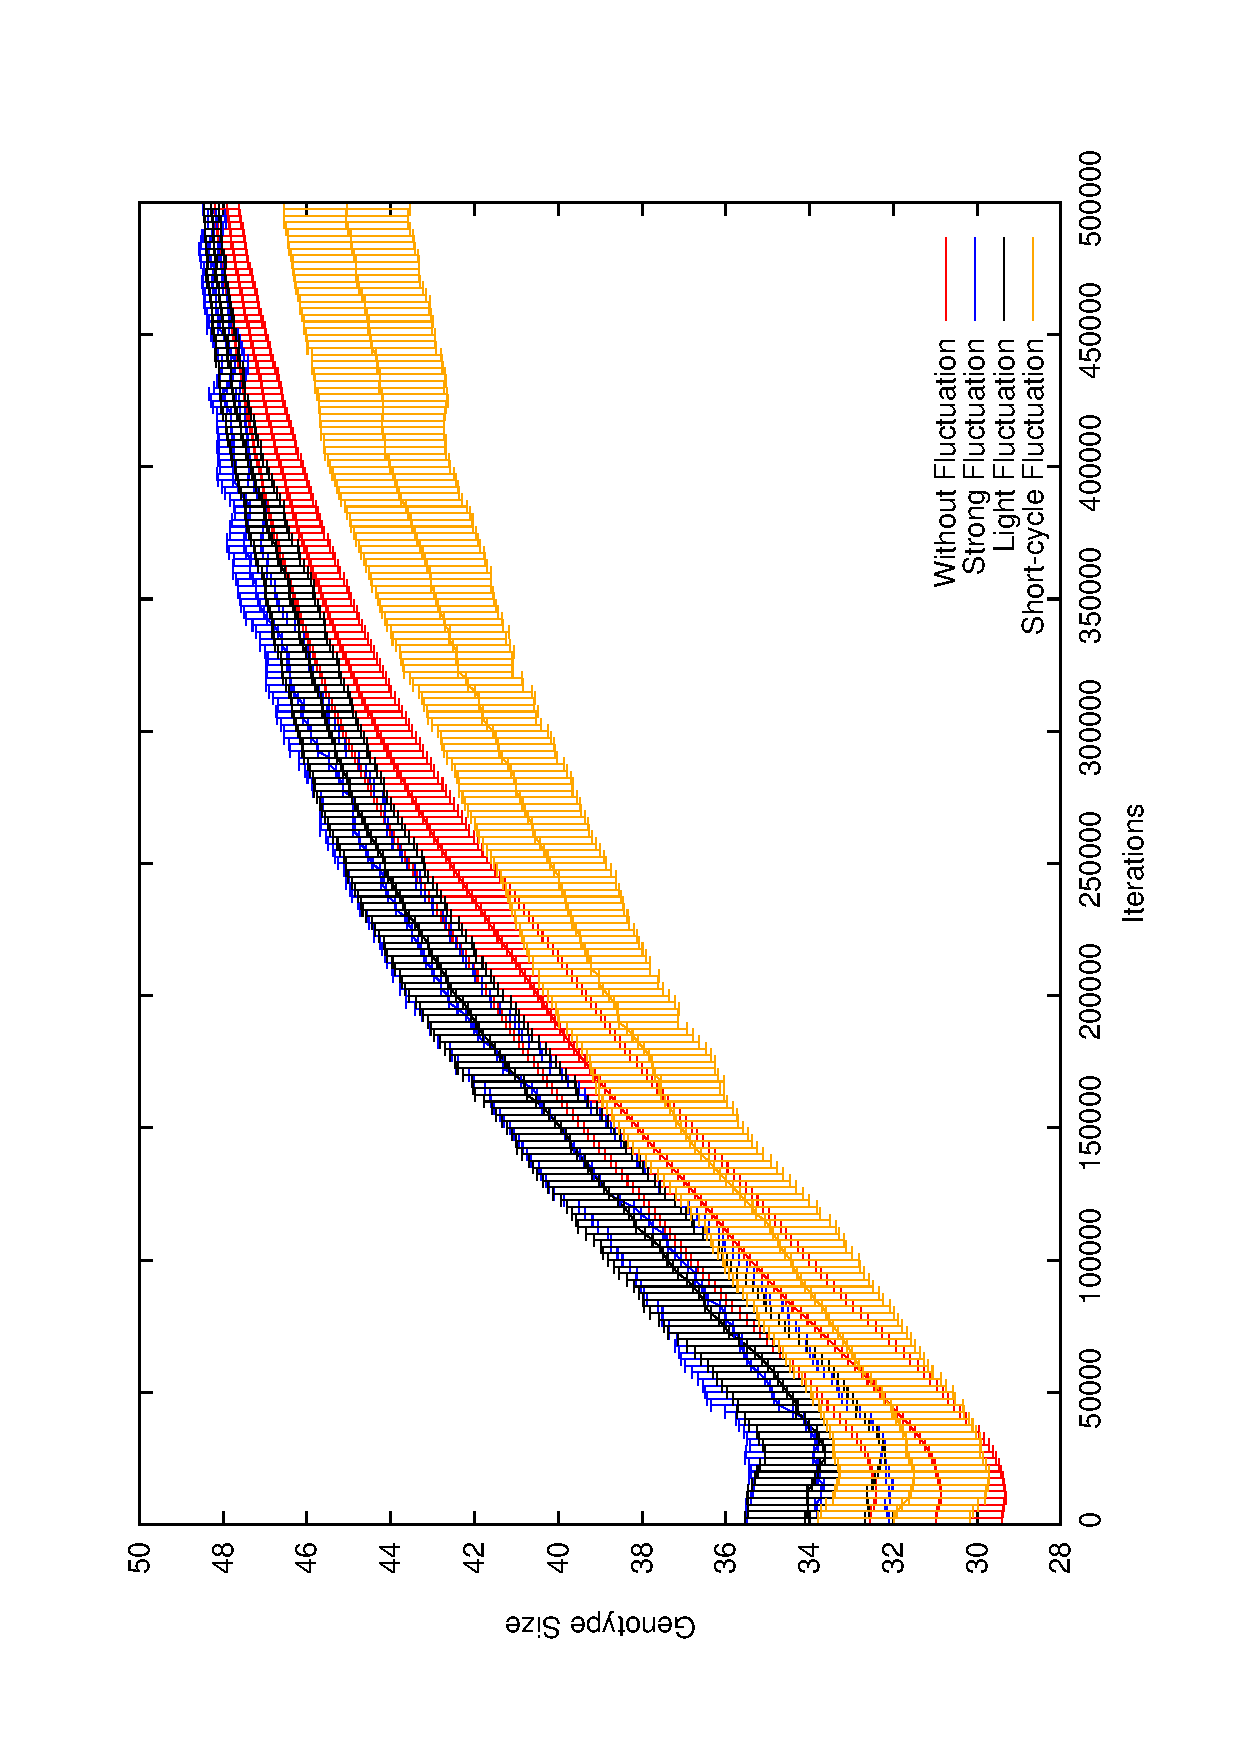
\includegraphics[width=0.7\columnwidth, angle =-90 ]{img/Size}
\caption{\textbf{Size of genotypes}. 
}
\label{fig:Size}
\end{figure}

\begin{figure}[h]
\centering
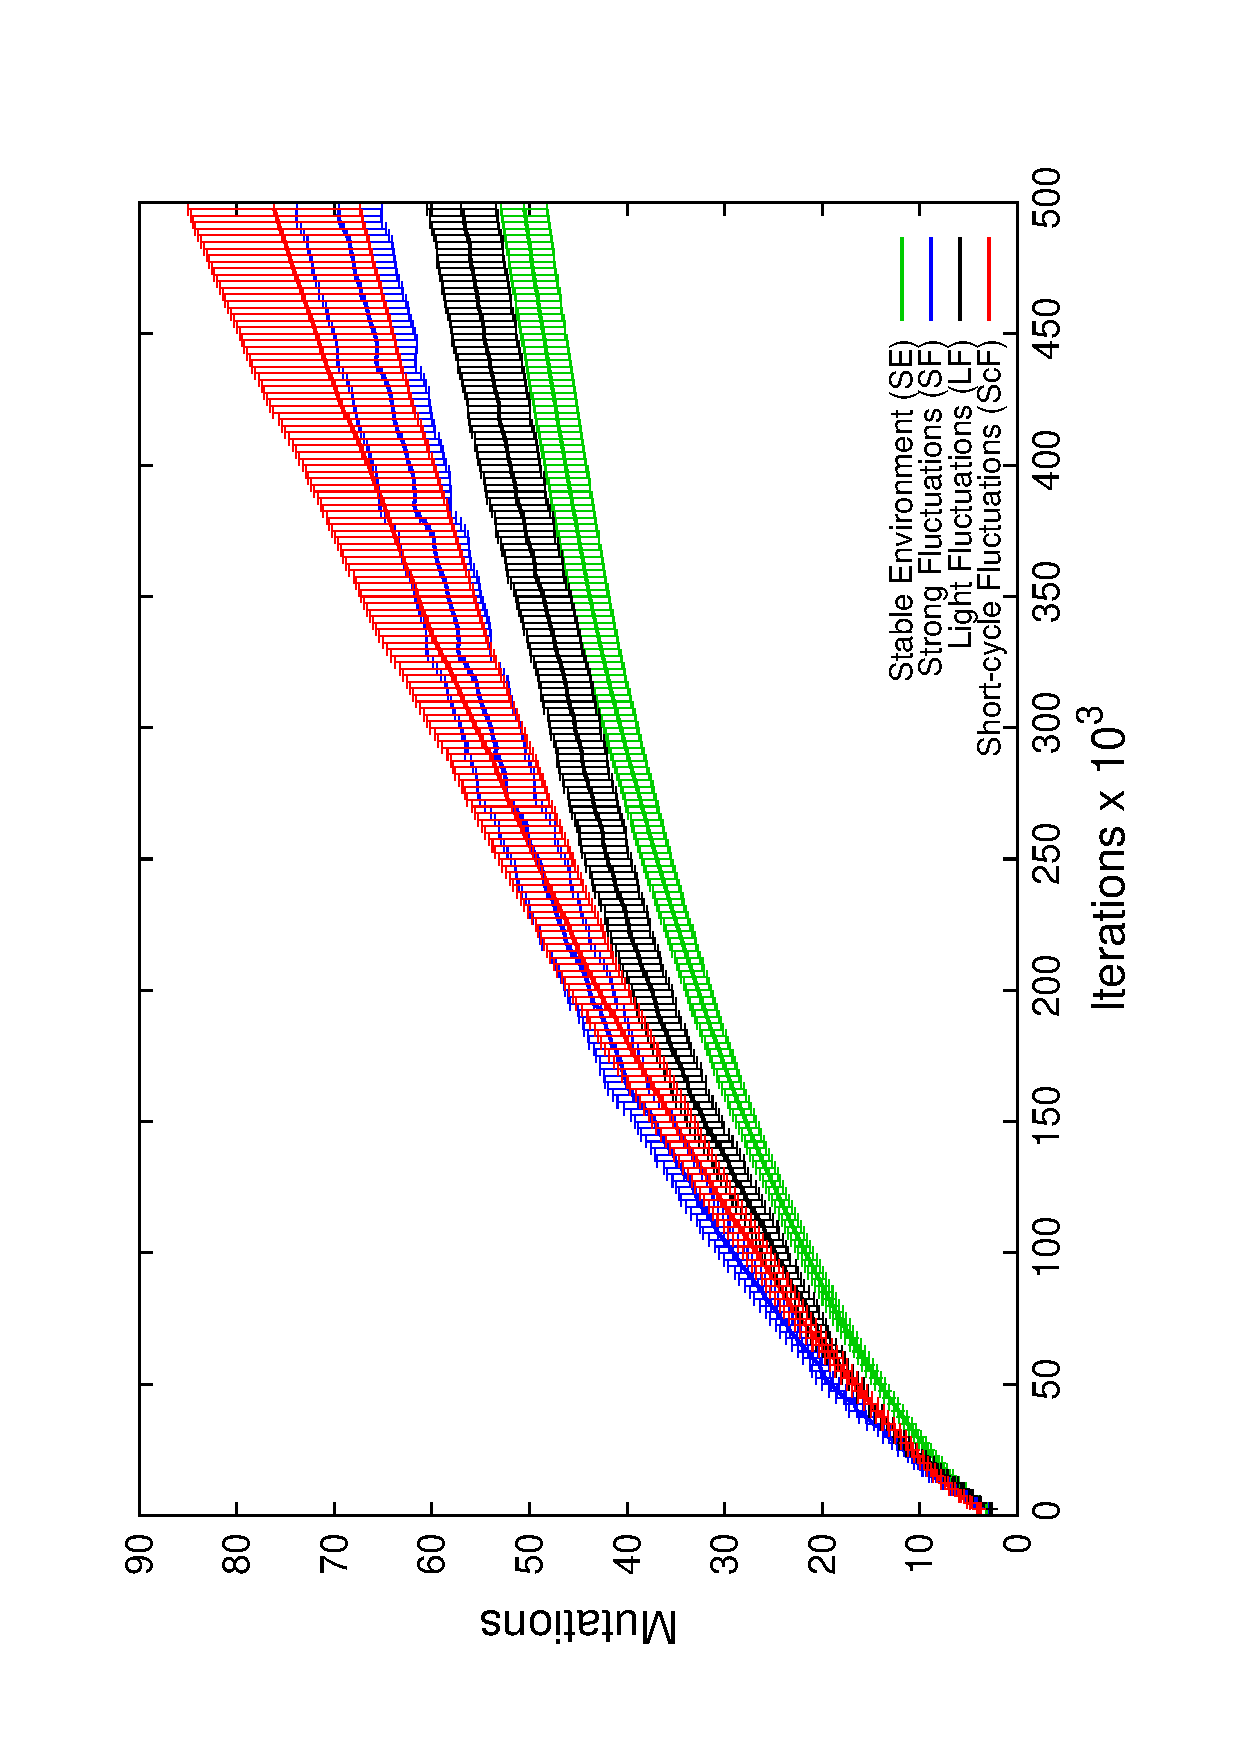
\includegraphics[width=0.7\columnwidth, angle =-90 ]{img/Mutations}
\caption{\textbf{Mutations of genotypes}.
}
\label{fig:Mutations}
\end{figure}

\subsection{Phenotypic Comparison}
Figure~\ref{fig:disimilar} depict phenotypic comparison of disimilar environment, one can see that the impact of environmental fluctuations decreases for \emph{Short-cycle  Fluctuation} while it remains very high for other forms of environmental fluctuations. We also noted that the phenotypic difference fall quickly for \emph{Short-cycle fluctuations} and even became almost similar to that of the simulation without fluctuation from iteration 20000. This suggests a selection of a single phenotype, robust in both environments. Figure~\ref{fig:disimilar} depict phenotypic comparison of similar environmen

\begin{figure}[h]
\centering
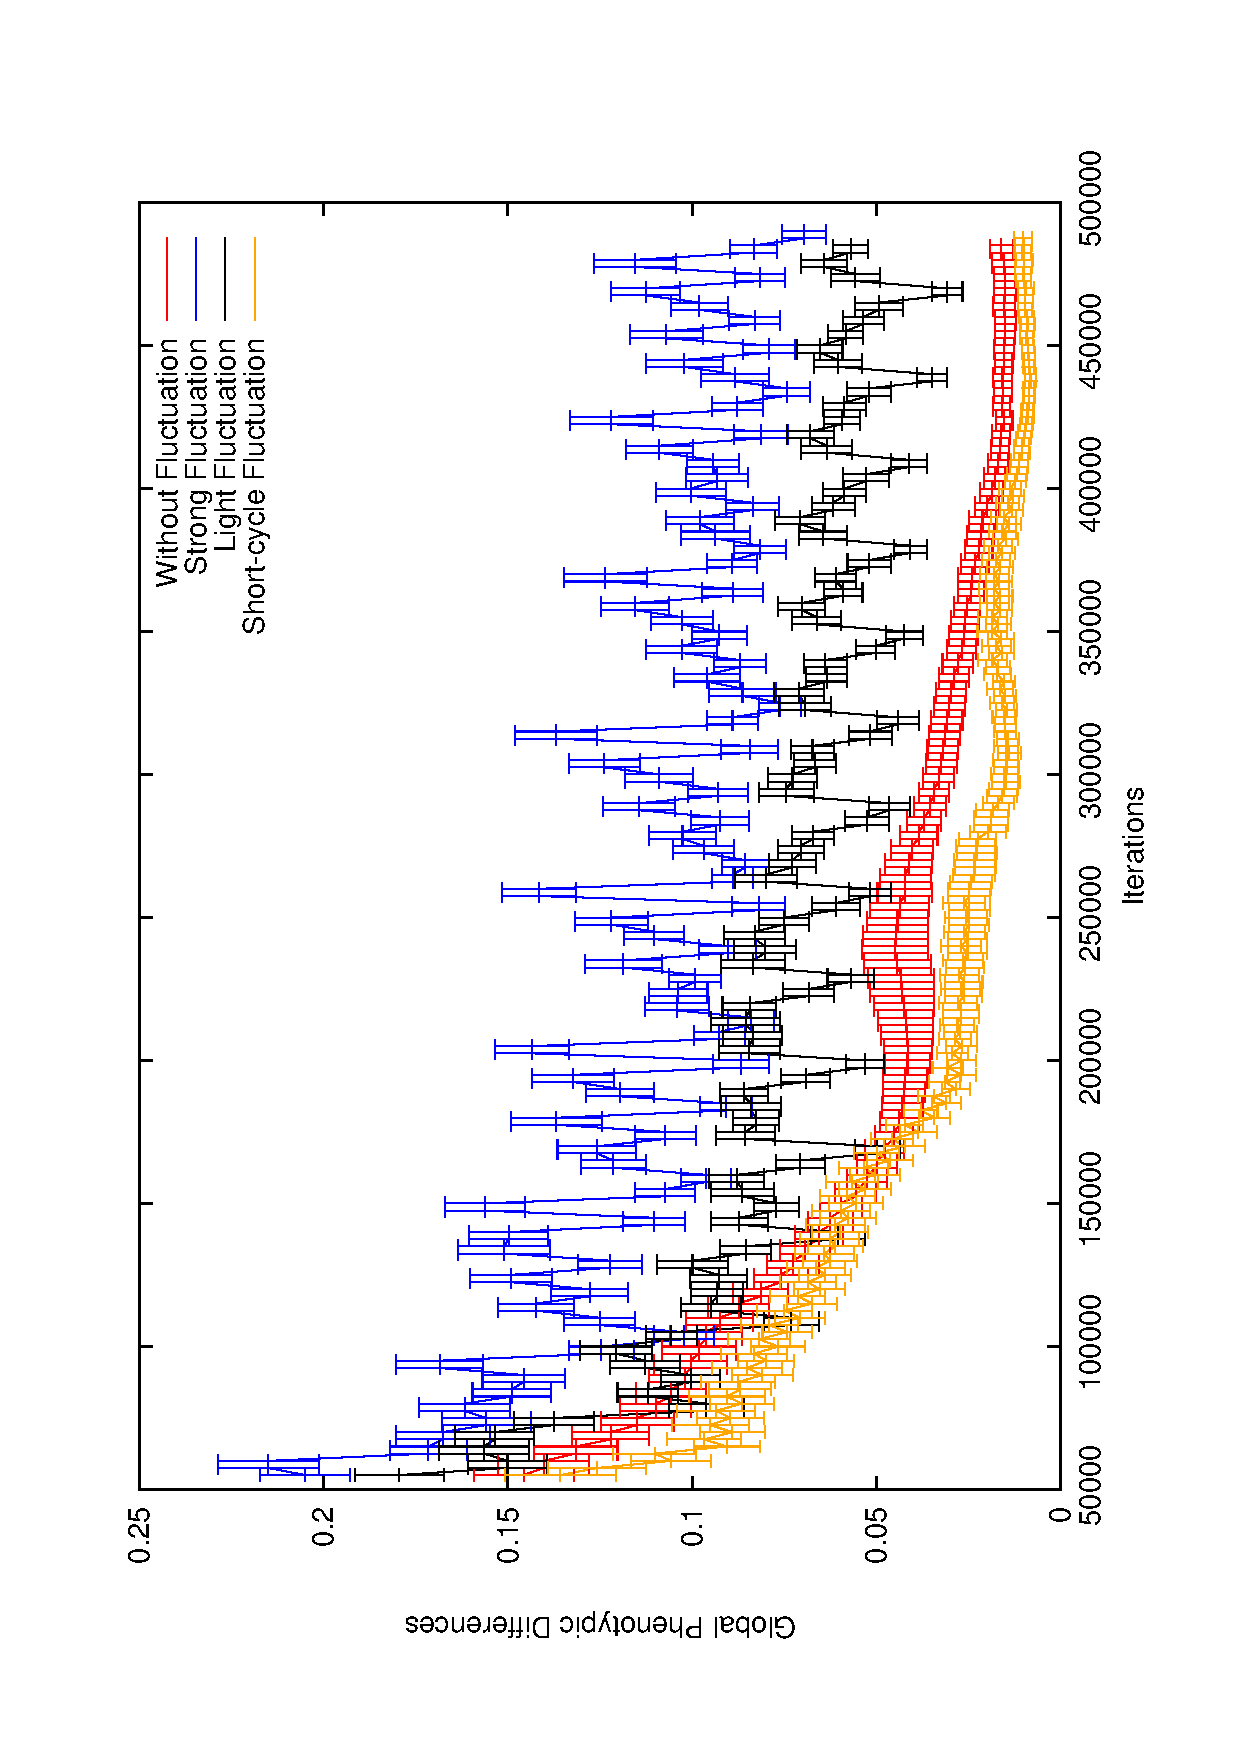
\includegraphics[width=0.7\columnwidth, angle =-90 ]{img/diffProp}
\caption{\textbf{phenotypic comparison of disimilar environment}.
}
\label{fig:disimilar}
\end{figure}

\begin{figure}[h]
\centering
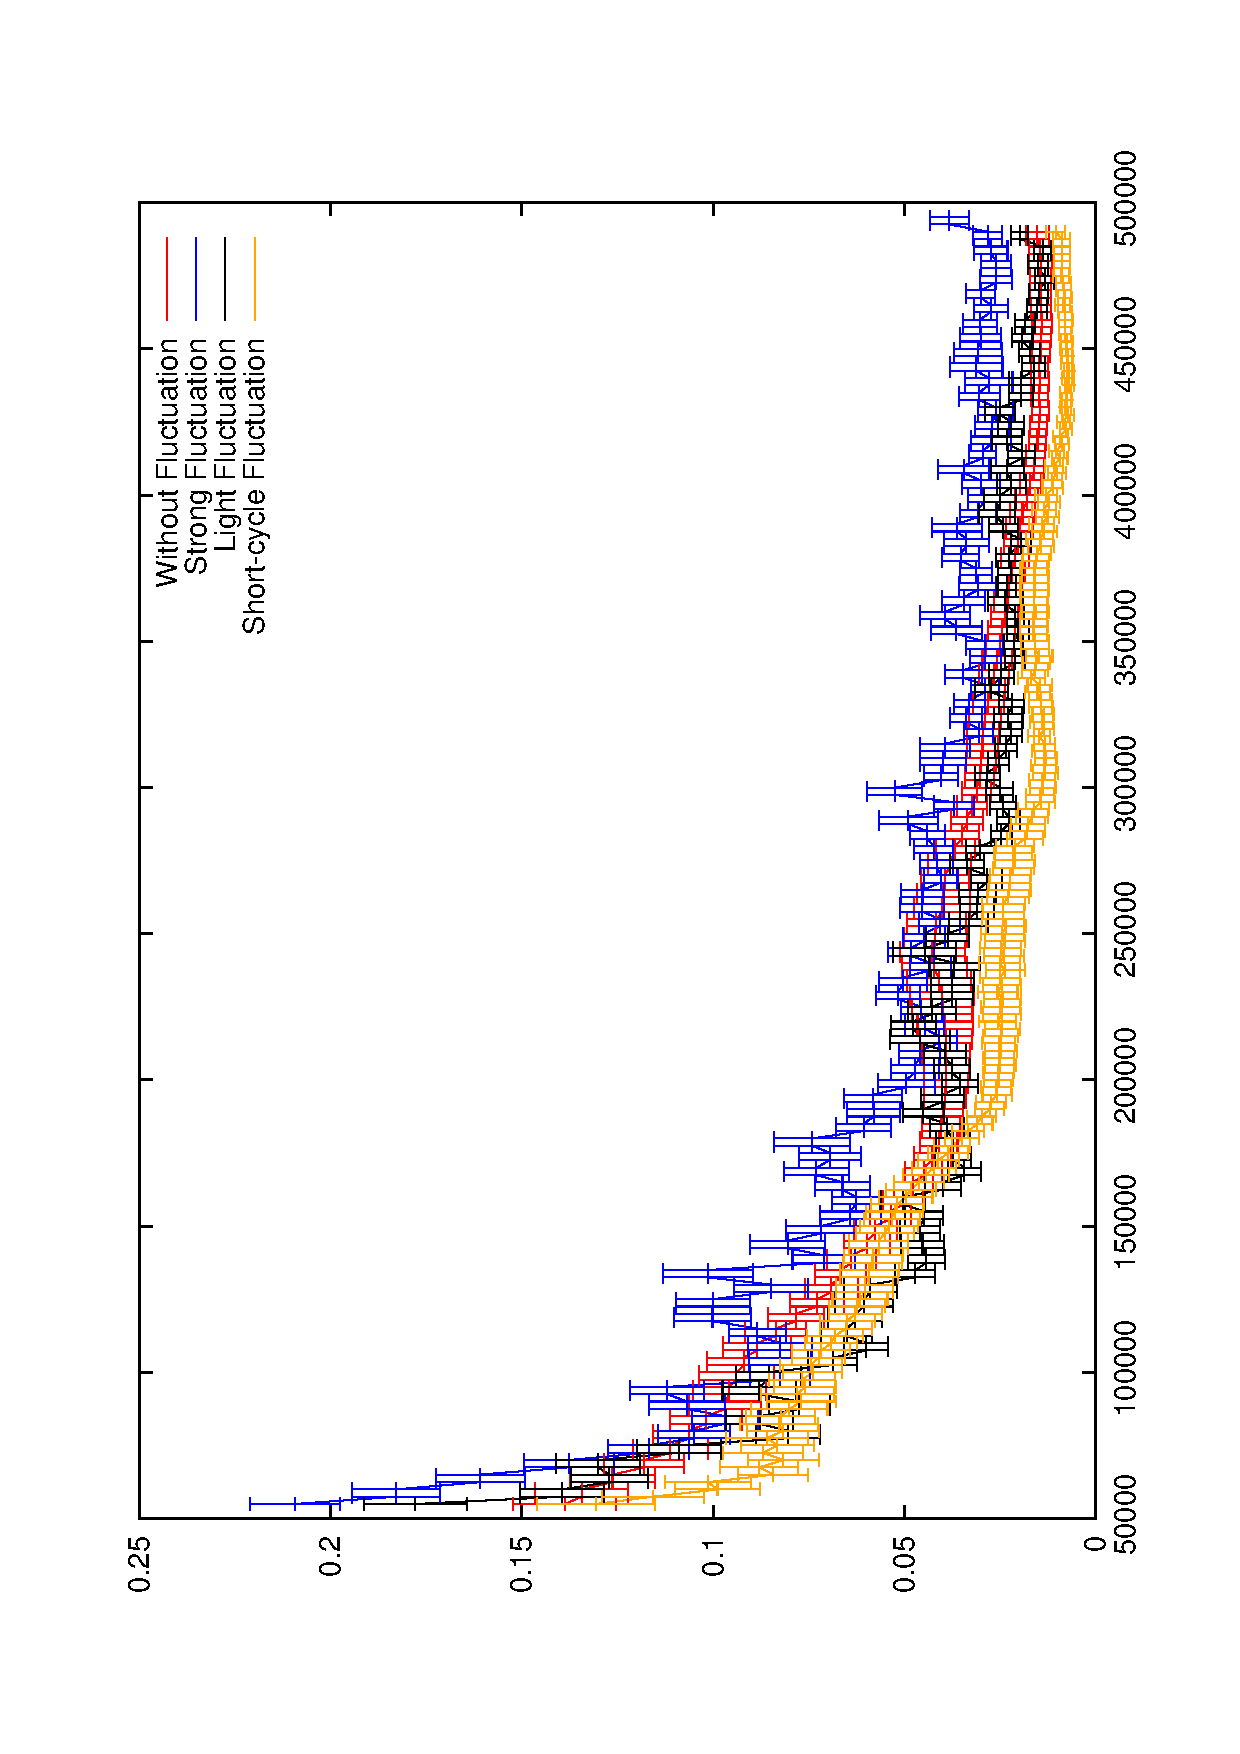
\includegraphics[width=0.7\columnwidth, angle =-90 ]{img/ProgressProp}
\caption{\textbf{phenotypic comparison of similar environment} : Here one can see that the impact of environmental fluctuations decreases for \emph{Short-cycle  Fluctuation} and  \emph{Light  Fluctuation}  while it remains very high for other forms of environmental fluctuations.
}
\label{fig:similar}
\end{figure}

\subsection{Success Rate}
Success rates of genotypes in different homogenous simulations are reported in Table \ref{tab:scstable} to \ref{tab:scstrong} using normal approximation interval with a confidence of 95\%. Looking at the different success rates we can first order the different tested environment by increasing difficulty : \em{Stable Environment}; \em{Short-cycle Fluctuations}; \em{Light Fluctuations} ; \em{Strong Fluctuations}. The fact that the \em{stable environment} offers the lowest challenge is not surprising. Similarly the fact that \em{Light Fluctuations} are less difficult than \em{Strong fluctuations} is quite expected. We believe that the slightest difficulty in \em{Short-cycle Fluctuations} than in \em{Light Fluctuations} is due to the reduced number of different environment in \em{Short-cycle Fluctuations} and in particular the fact that in this configuration one of the living state is always allowed. It is also noteworthy that while individuals from \em{Strong and Light Fluctuations} seem relatively robust in various environmental configurations while those from \em{Short-cycle Fluctuations} doesn't seem robust outside environmental conditions in which they evolved. Moreover these same individuals are the only ones that do not reach a 100\% survival ratio in a stable environment from 102500 iteration.

\begin{table*}
\caption{Success Rate of genotypes in homogenous test with stable environment.\label{tab:scstable}}
\scriptsize
\begin{tabular}{ccccccc}
\toprule%
{\textbf{Collection}} & {\textbf{2500}} & \textbf{102500} & \textbf{202500} &\textbf{302500} &\textbf{402500} &\textbf{500000} \tabularnewline
\toprule%
\textbf{Stable Environment} & $88\%\pm9\%$ & $100\%\pm0\%$ & $100\%\pm0\%$ & $100\%\pm0\%$ & $100\%\pm0\%$ & $100\%\pm0\%$\tabularnewline

\textbf{Short-cycle Fluctuations} & $98\%\pm4\%$ & $88\%\pm9\%$ & $88\%\pm9\%$ & $88\%\pm9\%$ & $88\%\pm9\%$ & $88\%\pm9\%$\tabularnewline

\textbf{Light Fluctuations} & $94\%\pm6\%$ & $100\%\pm0\%$ & $100\%\pm0\%$ & $100\%\pm0\%$ & $100\%\pm0\%$ & $100\%\pm0\%$\tabularnewline

\textbf{Strong Fluctuations} & $96\%\pm5\%$ & $100\%\pm0\%$ & $100\%\pm0\%$ & $100\%\pm0\%$ & $100\%\pm0\%$ & $100\%\pm0\%$\tabularnewline

\bottomrule%
\end{tabular}%
\end{table*} 

\begin{table*}
\caption{Success Rate of genotypes in homogenous test with Short Cycle Fluctuations.\label{tab:scshort}}
\scriptsize
\begin{tabular}{ccccccc}
\toprule%
{\textbf{Collection}} & {\textbf{2500}} & \textbf{102500} & \textbf{202500} &\textbf{302500} &\textbf{402500} &\textbf{500000} \tabularnewline
\toprule%

\textbf{Stable Environment} & $37\%\pm13\%$ & $55\%\pm14\%$ & $45\%\pm14\%$ & $55\%\pm14\%$ & $57\%\pm14\%$ & $47\%\pm14\%$ \tabularnewline
\textbf{Short-cycle Fluctuations} & $33\%\pm13\%$ & $88\%\pm9\%$ & $88\%\pm9\%$ & $88\%\pm9\%$ & $88\%\pm9\%$ & $88\%\pm9\%$ \tabularnewline
\textbf{Light Fluctuations} &$29\%\pm13\%$ & $61\%\pm13\%$ & $69\%\pm13\%$ & $69\%\pm13\%$ & $84\%\pm10\%$ & $82\%\pm10\%$ \tabularnewline
\textbf{Strong Fluctuations} &$40\%\pm14\%$ & $80\%\pm11\%$ & $96\%\pm5\%$ & $96\%\pm5\%$ & $90\%\pm8\%$ & $86\%\pm9\%$\tabularnewline

\bottomrule%
\end{tabular}%
\end{table*} 

\begin{table*}
\caption{Success Rate of genotypes in homogenous test with Light Fluctuations.\label{tab:scslight}}
\scriptsize
\begin{tabular}{ccccccc}
\toprule%
{\textbf{Collection}} & {\textbf{2500}} & \textbf{102500} & \textbf{202500} &\textbf{302500} &\textbf{402500} &\textbf{500000} \tabularnewline
\toprule%

\textbf{Stable Environment} & $20\%\pm11\%$ & $59\%\pm14\%$ & $65\%\pm13\%$ & $73\%\pm12\%$ & $73\%\pm12\%$ & $67\%\pm13\%$\tabularnewline
\textbf{Short-cycle Fluctuations} & $18\%\pm10\%$ & $20\%\pm11\%$ & $14\%\pm9\%$ & $10\%\pm8\%$ & $8\%\pm7\%$ & $6\%\pm6\%$\tabularnewline
\textbf{Light Fluctuations} &$20\%\pm11\%$ & $90\%\pm8\%$ & $96\%\pm5\%$ & $98\%\pm4\%$ & $100\%\pm0\%$ & $98\%\pm4\%$\tabularnewline
\textbf{Strong Fluctuations} &$24\%\pm12\%$ & $90\%\pm8\%$ & $98\%\pm4\%$ & $96\%\pm5\%$ & $96\%\pm5\%$ & $100\%\pm0\%$\tabularnewline

\bottomrule%
\end{tabular}%
\end{table*} 

\begin{table*}
\caption{Success Rate of genotypes in homogenous test with Strong Fluctuations.\label{tab:scstrong}}
\scriptsize
\begin{tabular}{ccccccc}
\toprule%
{\textbf{Collection}} & {\textbf{2500}} & \textbf{102500} & \textbf{202500} &\textbf{302500} &\textbf{402500} &\textbf{500000} \tabularnewline
\toprule%

\textbf{Stable Environment} & $0\%\pm0\%$ & $16\%\pm10\%$ & $16\%\pm10\%$ & $14\%\pm9\%$ & $12\%\pm9\%$ & $12\%\pm9\%$\tabularnewline
\textbf{Short-cycle Fluctuations} & $0\%\pm0\%$ & $4\%\pm5\%$ & $2\%\pm4\%$ & $4\%\pm5\%$ & $0\%\pm0\%$ & $0\%\pm0\%$\tabularnewline
\textbf{Light Fluctuations} & $2\%\pm4\%$ & $16\%\pm10\%$ & $25\%\pm12\%$ & $29\%\pm13\%$ & $29\%\pm13\%$ & $45\%\pm14\%$\tabularnewline
\textbf{Strong Fluctuations} & $0\%\pm0\%$ & $31\%\pm13\%$ & $43\%\pm14\%$ & $55\%\pm14\%$ & $55\%\pm14\%$ & $55\%\pm14\%$\tabularnewline

\bottomrule%
\end{tabular}%
\end{table*} 

\subsection{Last iterations}





\begin{figure}[H]
\begin{subfigure}{.25\textwidth}
  \centering
  \includegraphics[width=.7\linewidth, angle =-90]{img/boxdensitystable.eps}
  \caption{Stable environment.}
  \label{fig:sfig1}
\end{subfigure}%
\begin{subfigure}{.25\textwidth}
  \centering
  \includegraphics[width=.7\linewidth, angle =-90]{img/boxdensityvariation.eps}
  \caption{Strong Fluctuation.}
  \label{fig:sfig2}
\end{subfigure}

\begin{subfigure}{.25\textwidth}
  \centering
  \includegraphics[width=.7\linewidth, angle =-90]{img/boxdensityvariationLight.eps}
  \caption{Light Fluctuation.}
  \label{fig:sfig2}
\end{subfigure}%
\begin{subfigure}{.25\textwidth}
  \centering
  \includegraphics[width=.7\linewidth, angle =-90]{img/boxdensityvariationSmall.eps}
  \caption{Small Fluctuation.}
  \label{fig:sfig1}
\end{subfigure}
\caption{Density of Genotype : Each genotype density is processed in four possible different environments.}
\label{fig:size}
\end{figure}

\begin{figure}[H]
\begin{subfigure}{.25\textwidth}
  \centering
  \includegraphics[width=.7\linewidth, angle =-90]{img/boxendingsFailedstable.eps}
  \caption{Stable environment.}
  \label{fig:sfig1}
\end{subfigure}%
\begin{subfigure}{.25\textwidth}
  \centering
  \includegraphics[width=.7\linewidth, angle =-90]{img/boxendingsFailedvariation.eps}
  \caption{Strong Fluctuation.}
  \label{fig:sfig2}
\end{subfigure}

\begin{subfigure}{.25\textwidth}
  \centering
  \includegraphics[width=.7\linewidth, angle =-90]{img/boxendingsFailedvariationLight.eps}
  \caption{Light Fluctuation.}
  \label{fig:sfig2}
\end{subfigure}%
\begin{subfigure}{.25\textwidth}
  \centering
  \includegraphics[width=.7\linewidth, angle =-90]{img/boxendingsFailedvariationSmall.eps}
  \caption{Small Fluctuation.}
  \label{fig:sfig1}
\end{subfigure}
\caption{Last iteration with living cells of density runs that didn't reach 60000 iterations. Note that \emph{Short-cycle Fluctuation} genotypes failures are concentrated around iteration 15000 on \emph{Light Fluctuation} density test and around iteration 25000 on \emph{Strong Fluctuation} density test.}
\label{fig:size}
\end{figure}